\documentclass[aspectratio=169, xcolor=table]{beamer}

\usepackage{calc}
\usepackage{graphicx}
\usepackage{mathtools}
\usepackage{siunitx}
\usepackage{tikz}

\graphicspath{{./images}}
\setbeamertemplate{navigation symbols}{}

\author{Chris Doble}
\date{}
\subtitle{Building a GPS receiver from scratch}
\title{Part 1: Introduction}
\usetheme{Madrid}

% Show the topics frame at the start of each section
\AtBeginSection[]
{
  \begin{frame}
    \frametitle{Topics}
    \tableofcontents[currentsection, subsubsectionstyle=hide]
  \end{frame}
}

% Show the topics frame at the start of each subsection
\AtBeginSubsection[]
{
  \begin{frame}
    \frametitle{Topics}
    \tableofcontents[currentsection, currentsubsection, subsubsectionstyle=hide]
  \end{frame}
}

\begin{document}

\frame{\titlepage}

{
    \usebackgroundtemplate{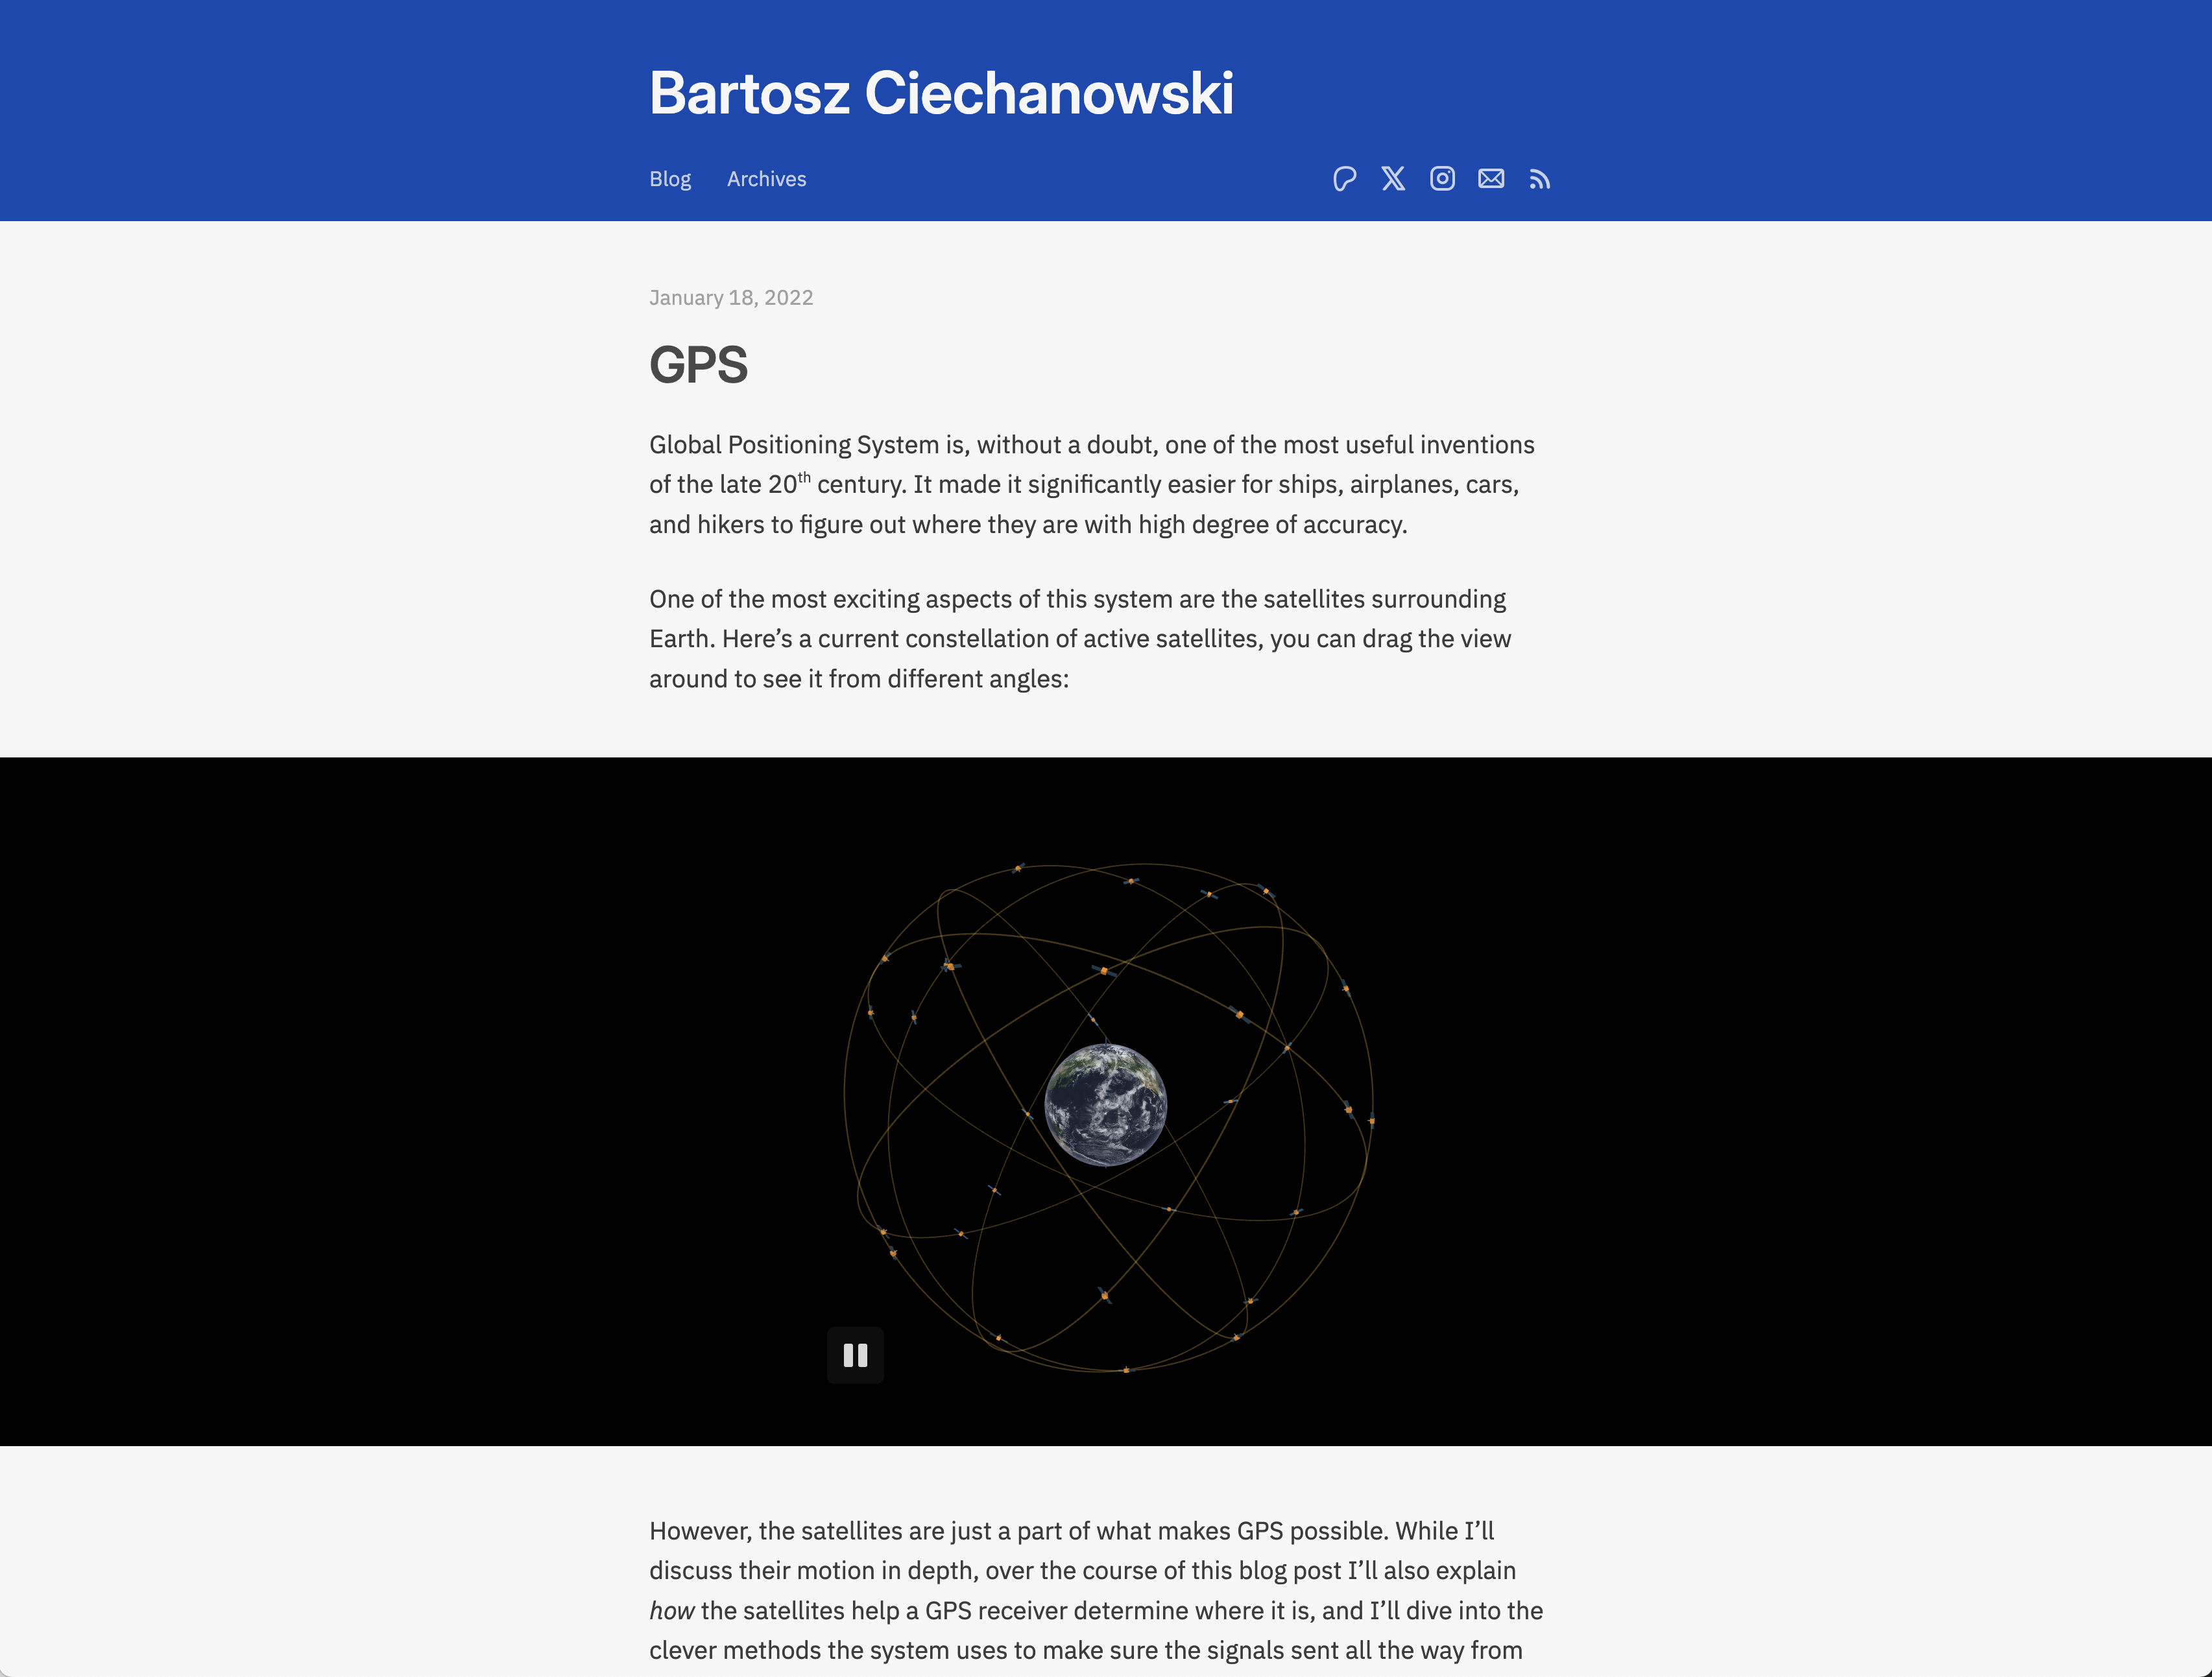
\includegraphics[width=\paperwidth]{1 bartosz.png}}
    \begin{frame}[b,plain]
        \colorbox{white}{https://ciechanow.ski/gps/}
        \vspace{0.3cm}
    \end{frame}
}

{
    \usebackgroundtemplate{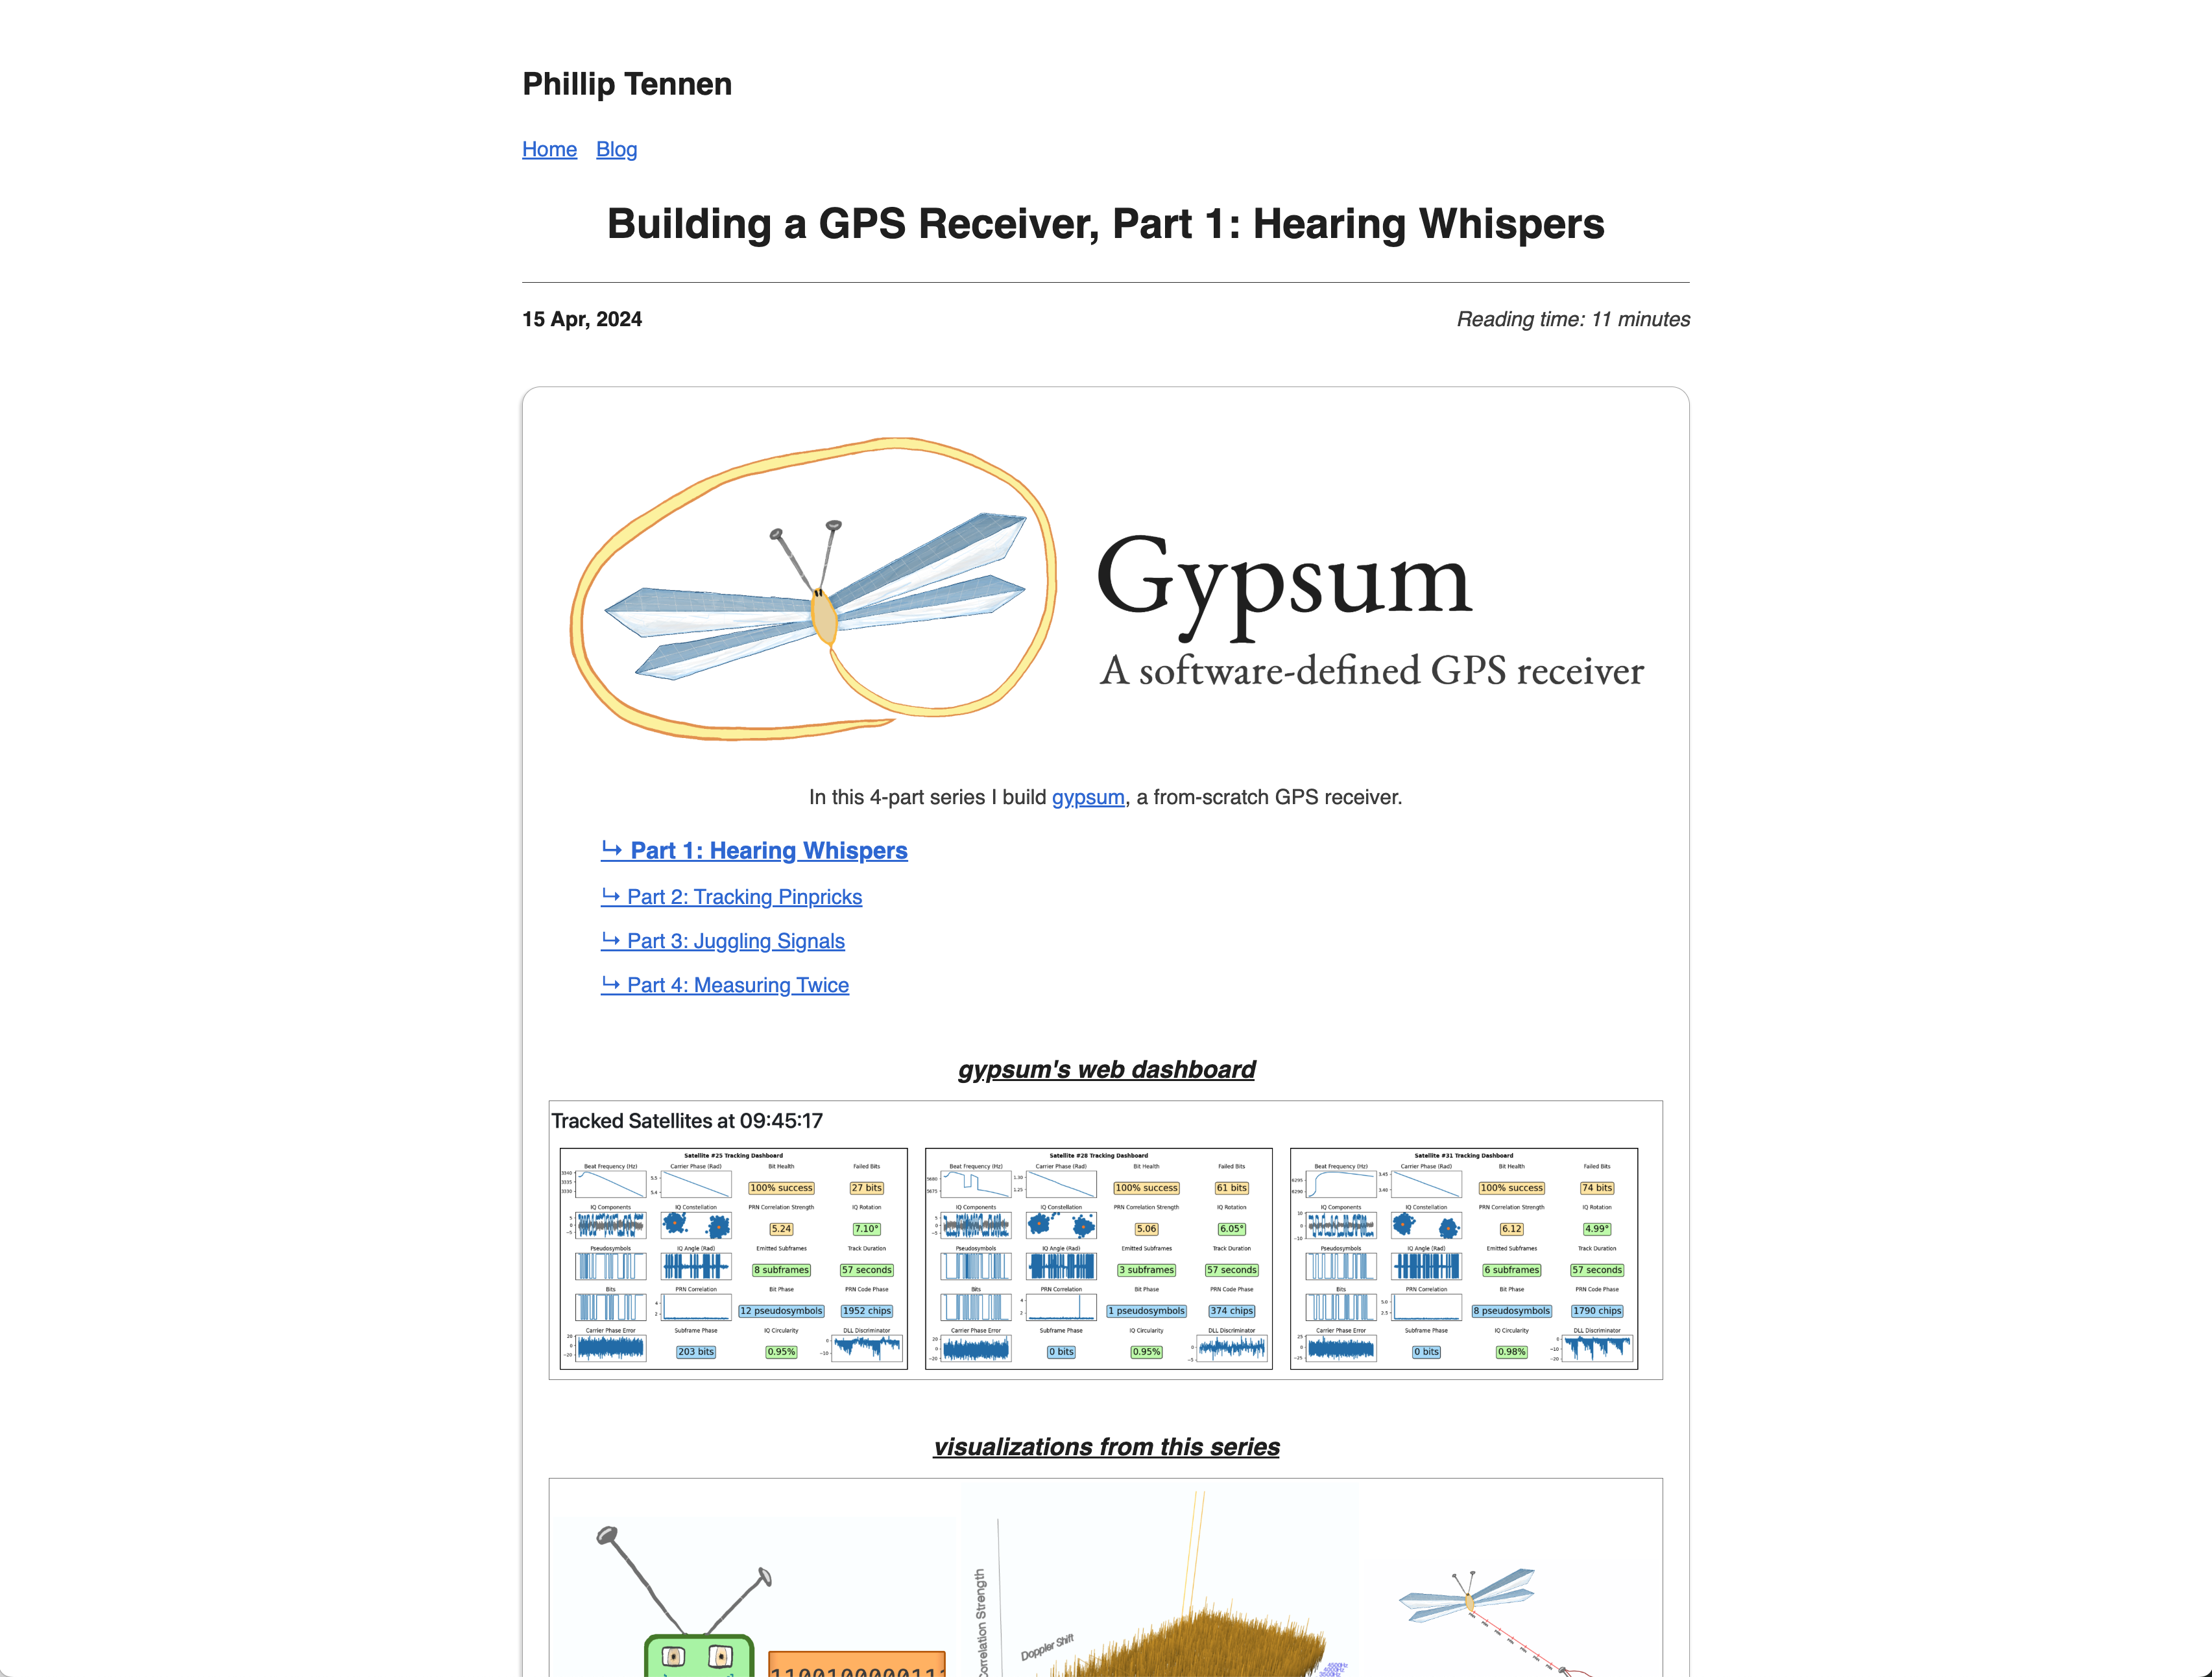
\includegraphics[width=\paperwidth]{2 phillip.png}}
    \begin{frame}[b,plain]
        \colorbox{black}{\color{white}{https://axleos.com/building-a-gps-receiver-part-1-hearing-whispers/}}
        \vspace{0.3cm}
    \end{frame}
}

\begin{frame}
    \frametitle{GPS receiver}

    \centering
    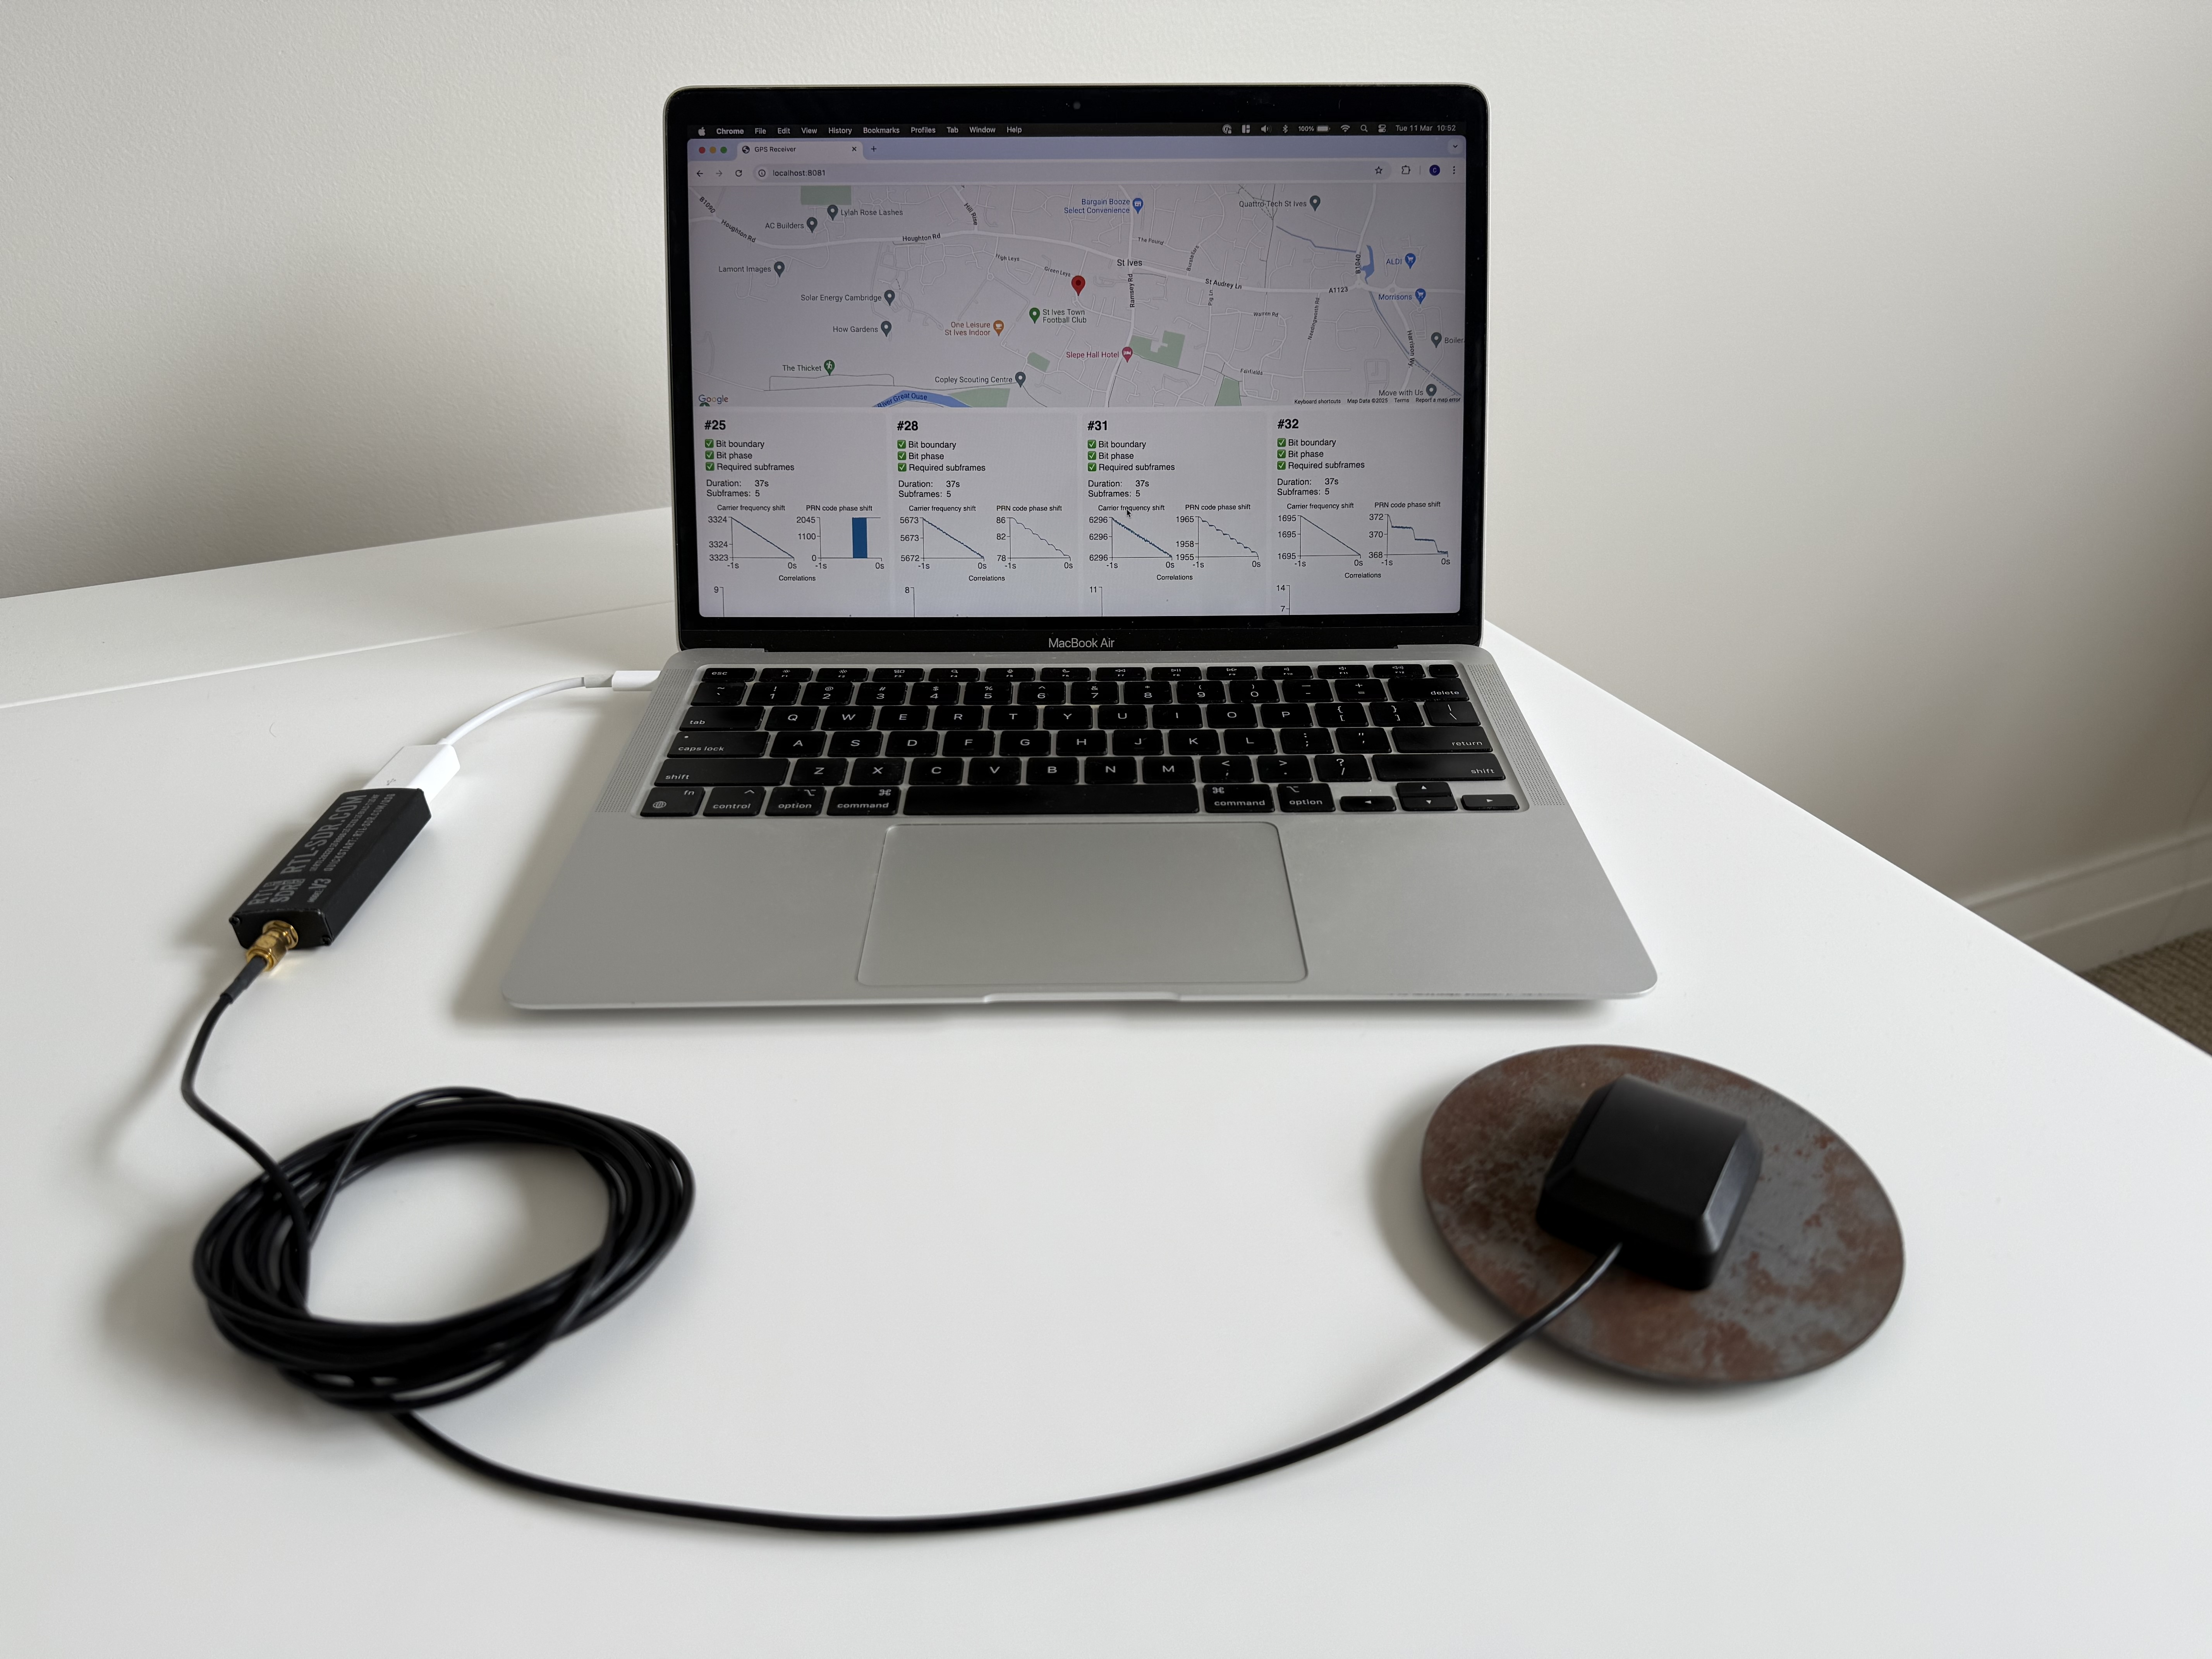
\includegraphics[width=\textwidth * 3 / 5]{9 setup.jpg}
\end{frame}

\begin{frame}
    \frametitle{Dashboard}

    \centering
    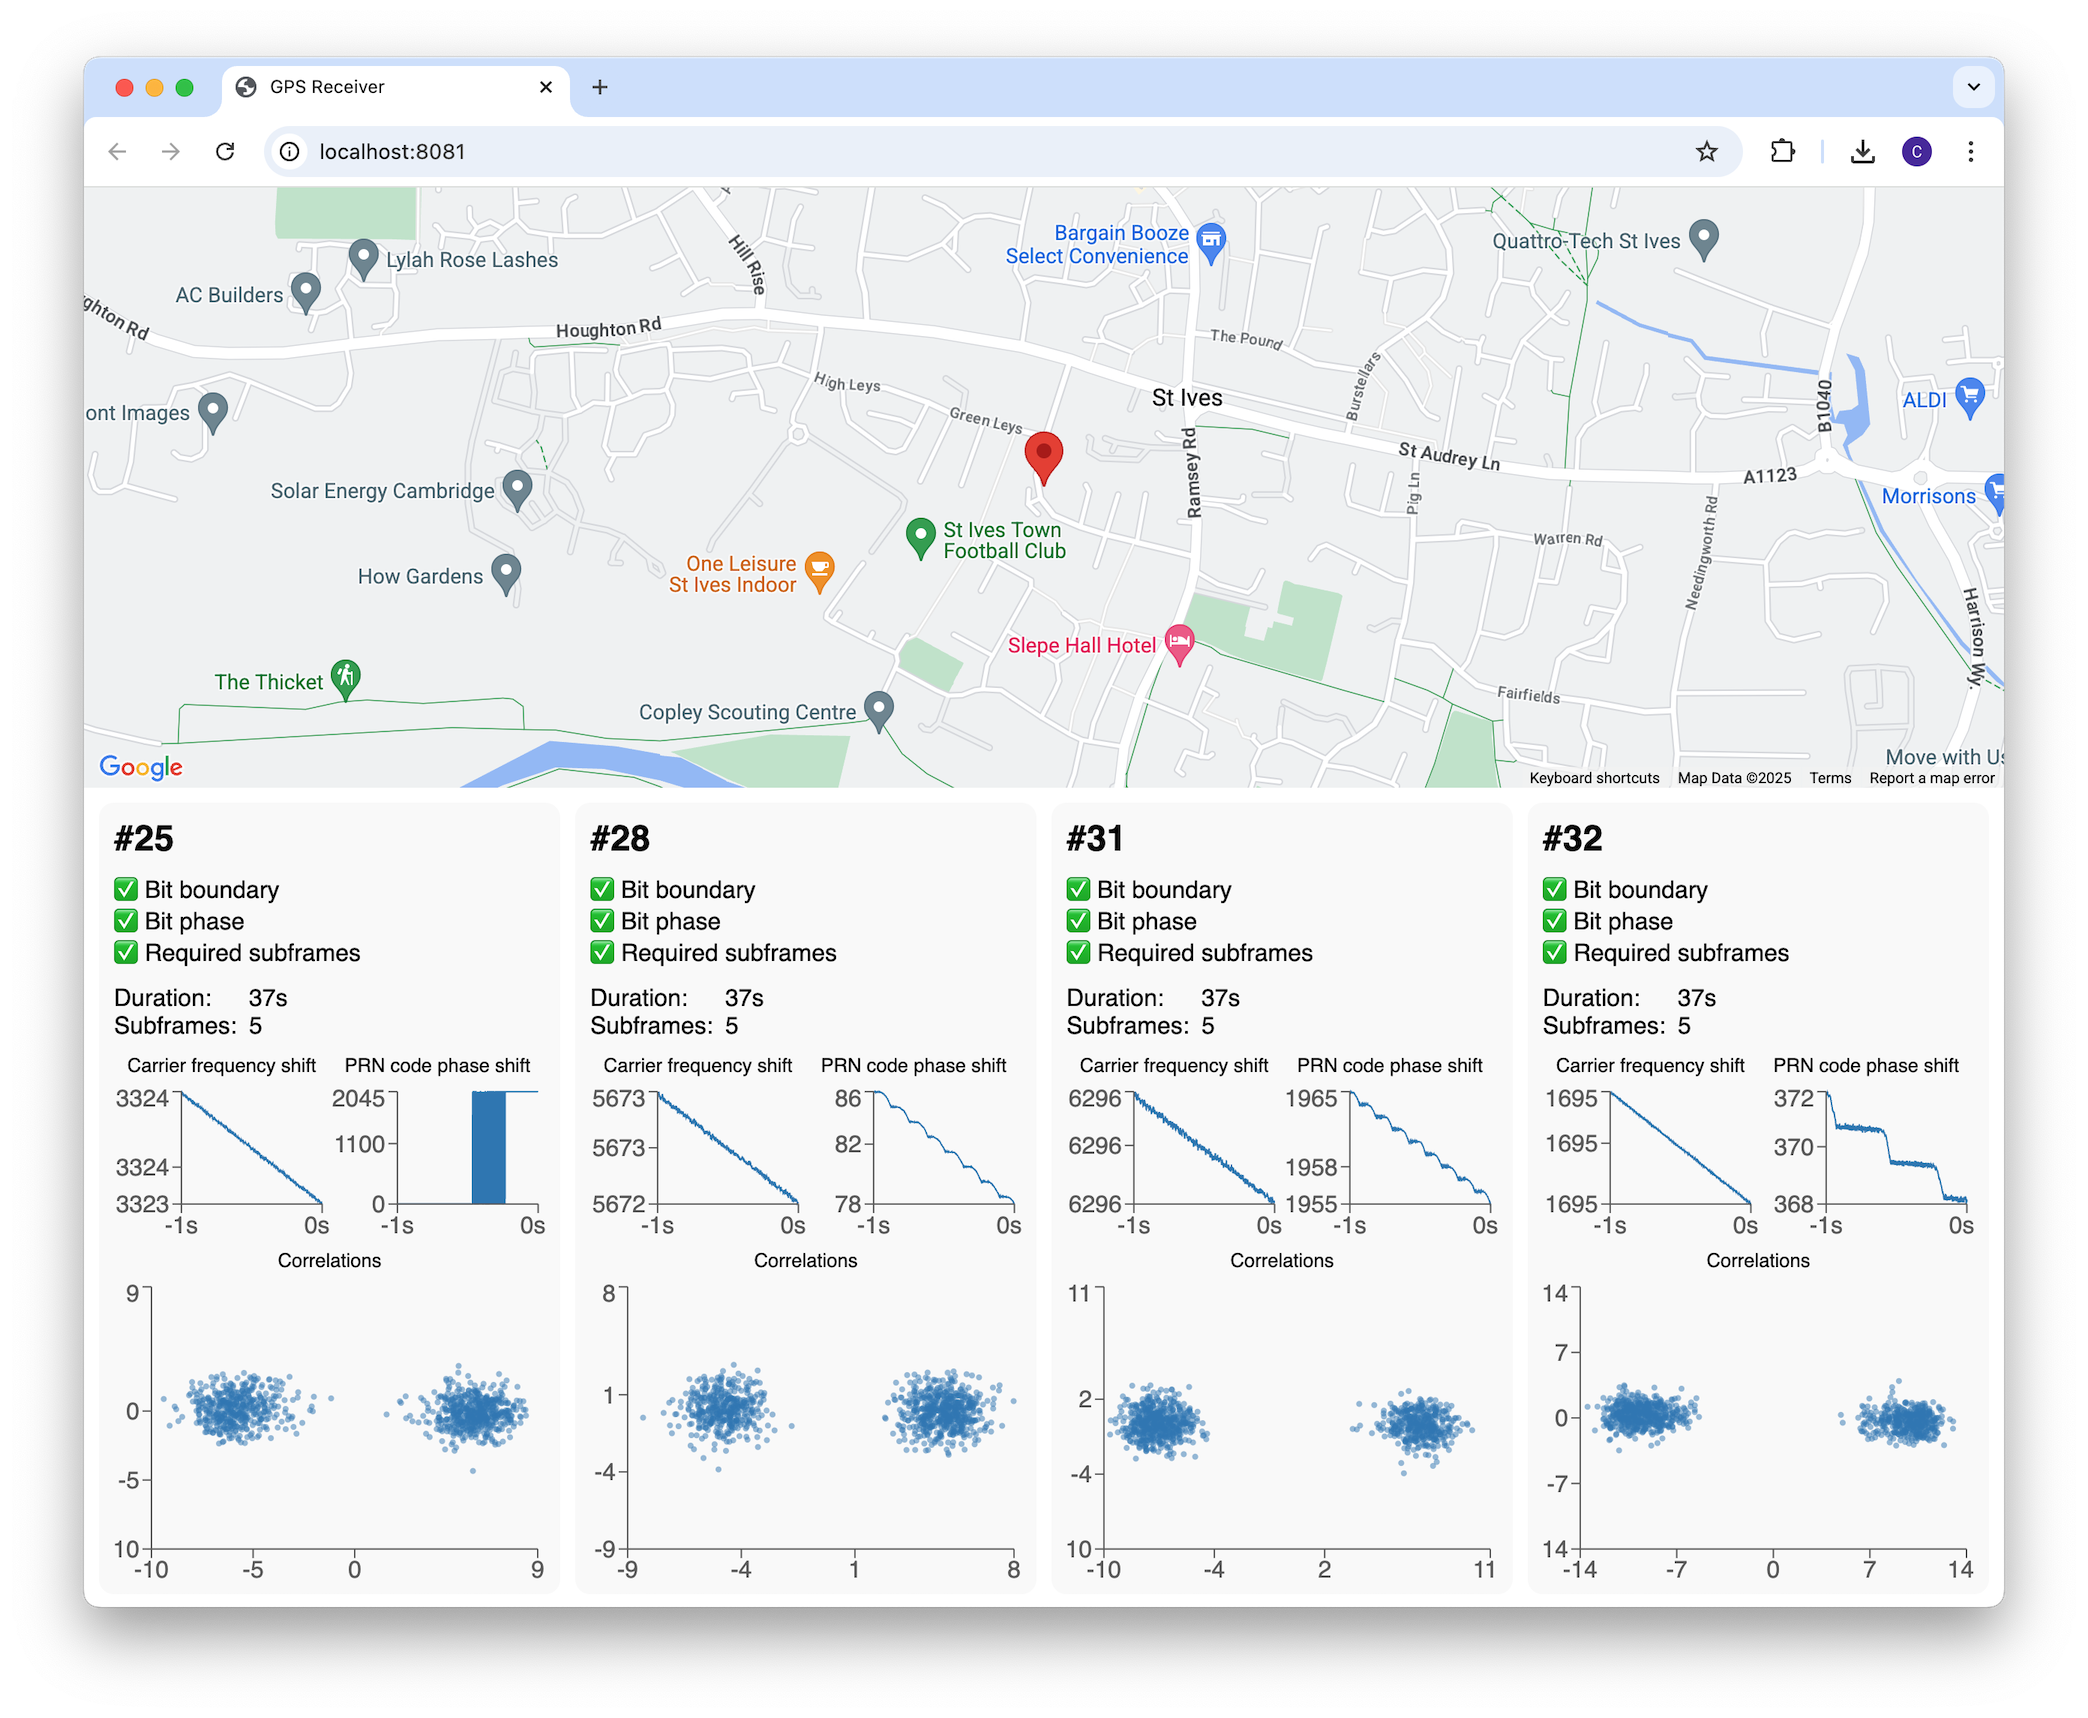
\includegraphics[width=\textwidth * 11 / 20]{10 dashboard.png}
\end{frame}

\begin{frame}
    \frametitle{Overview of GPS}

    \centering
    \only<1>{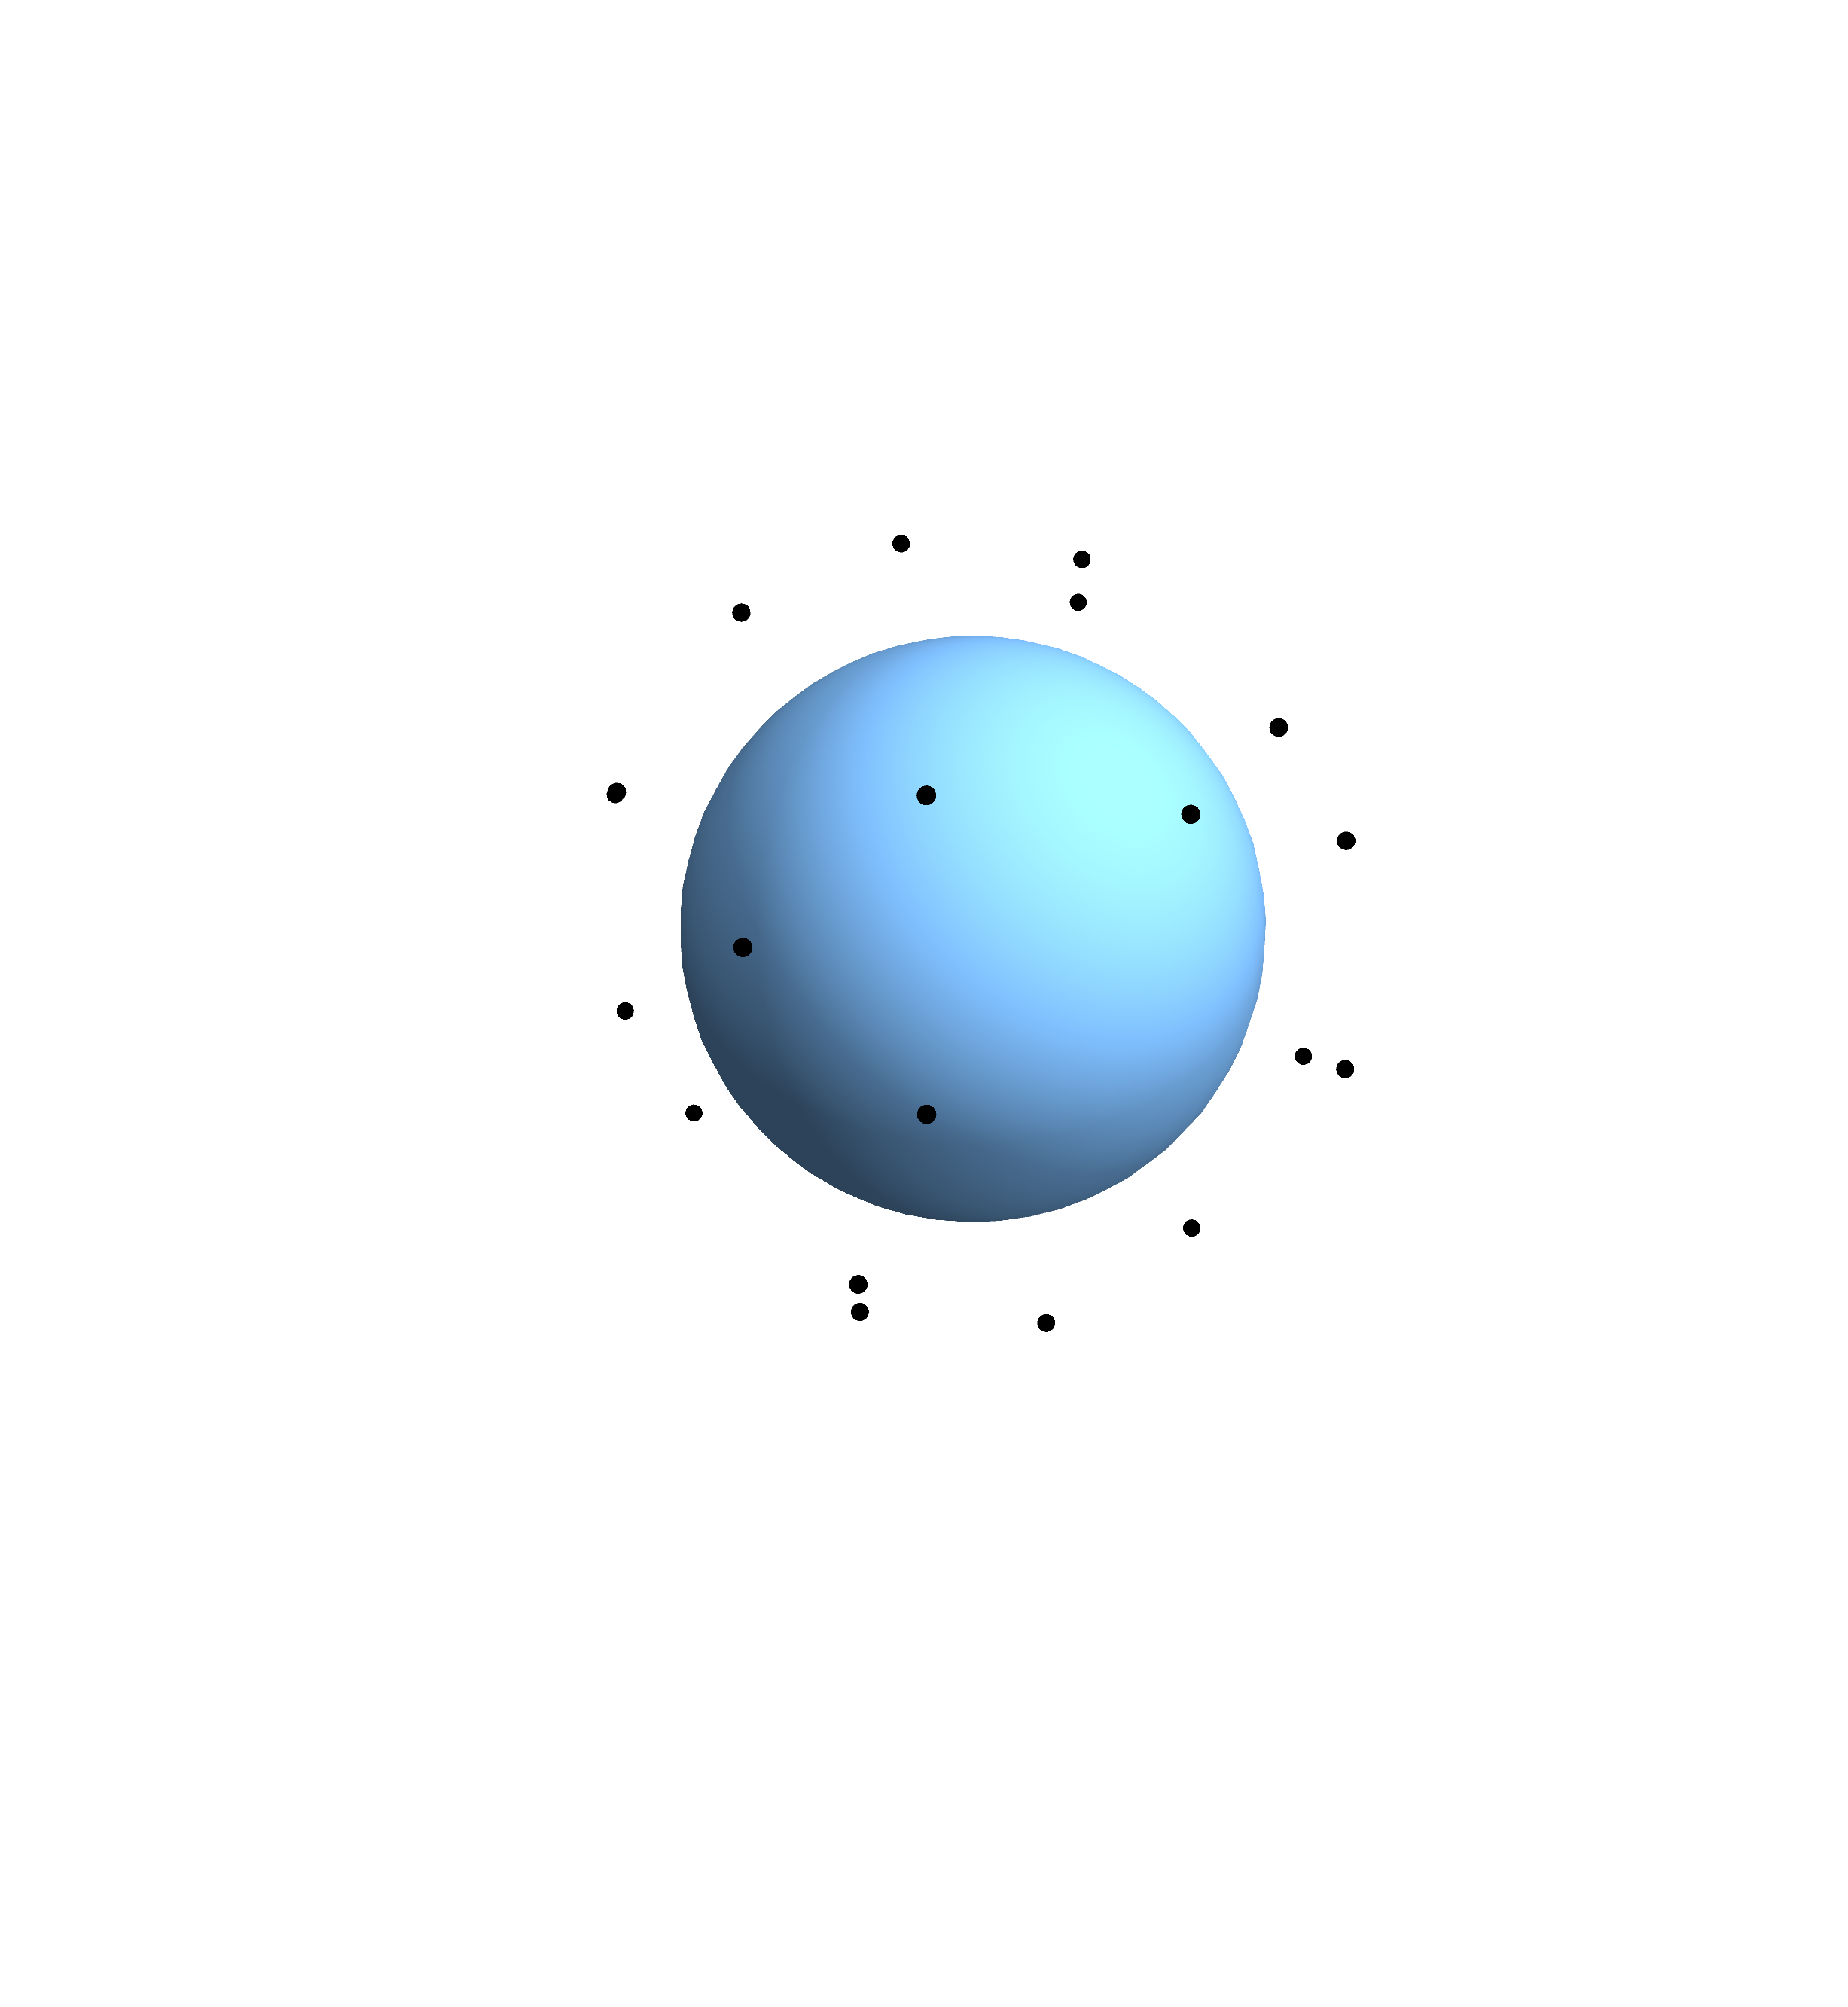
\includegraphics[clip, trim={13cm 15cm 8.5cm 11cm}, width=\textwidth * 35 / 100]{3 constellation.pdf}}%
    \only<2>{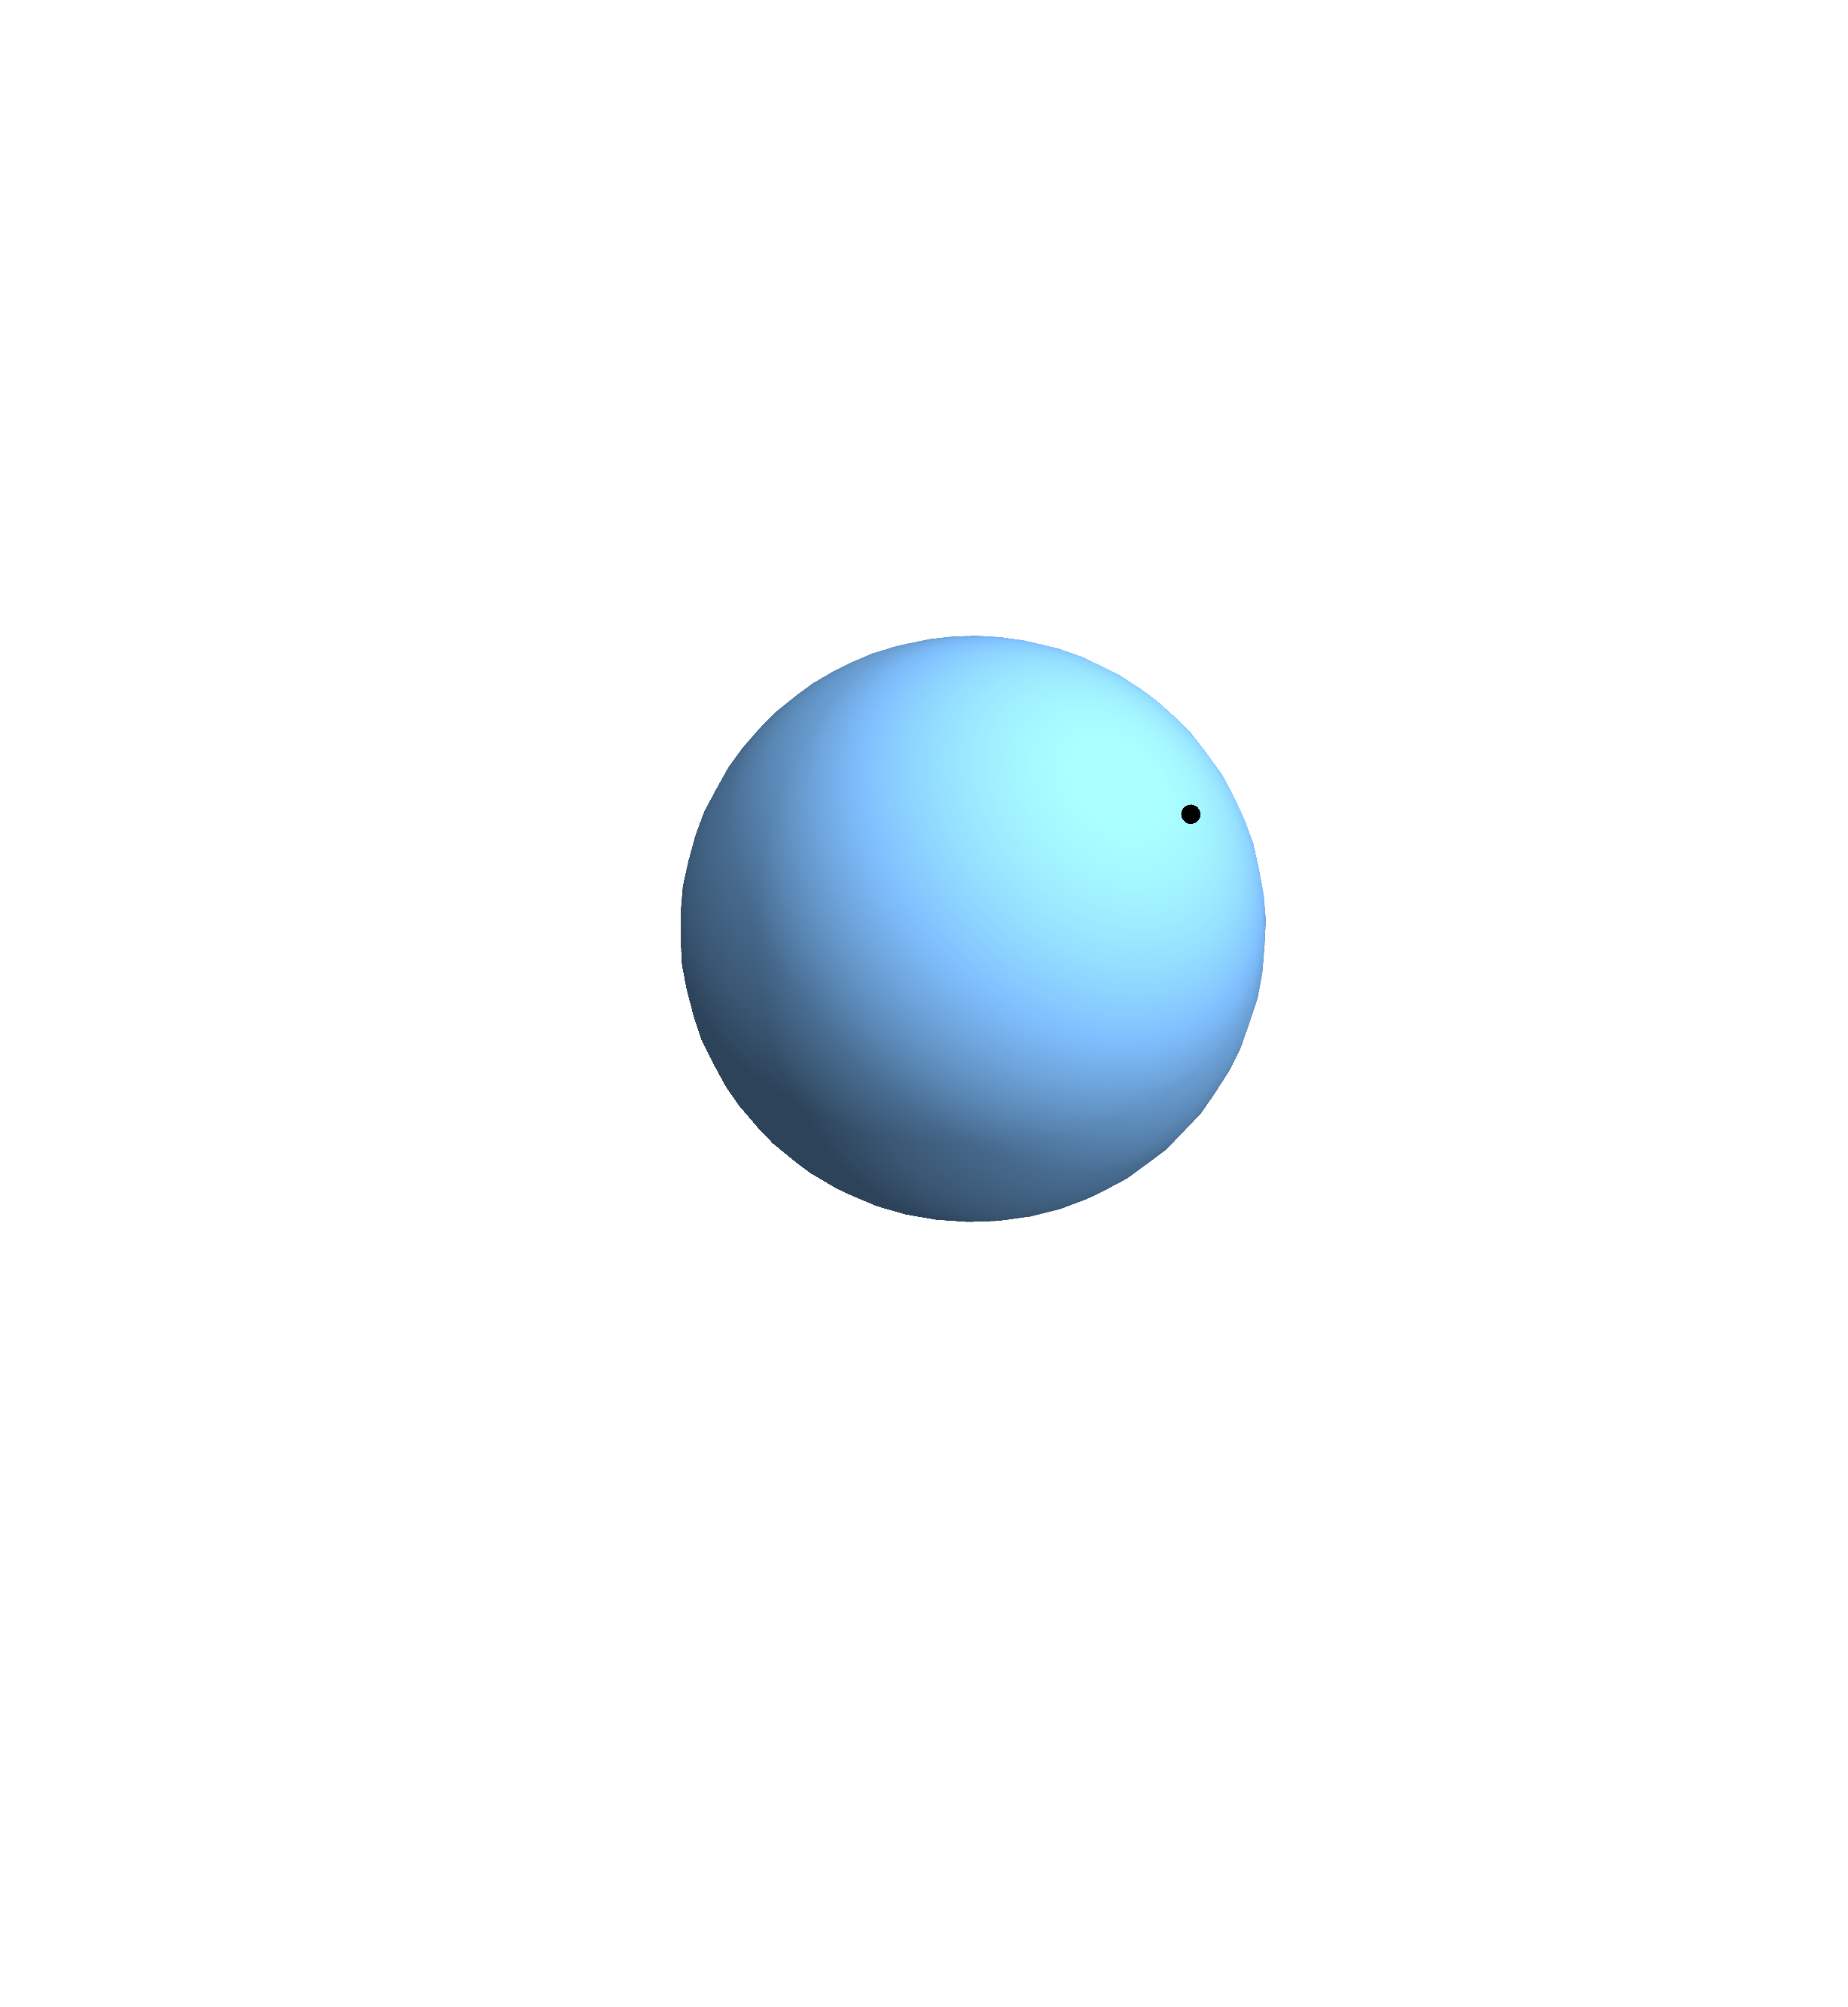
\includegraphics[clip, trim={13cm 15cm 8.5cm 11cm}, width=\textwidth * 35 / 100]{4 one satellite.pdf}}%
    \only<3-5>{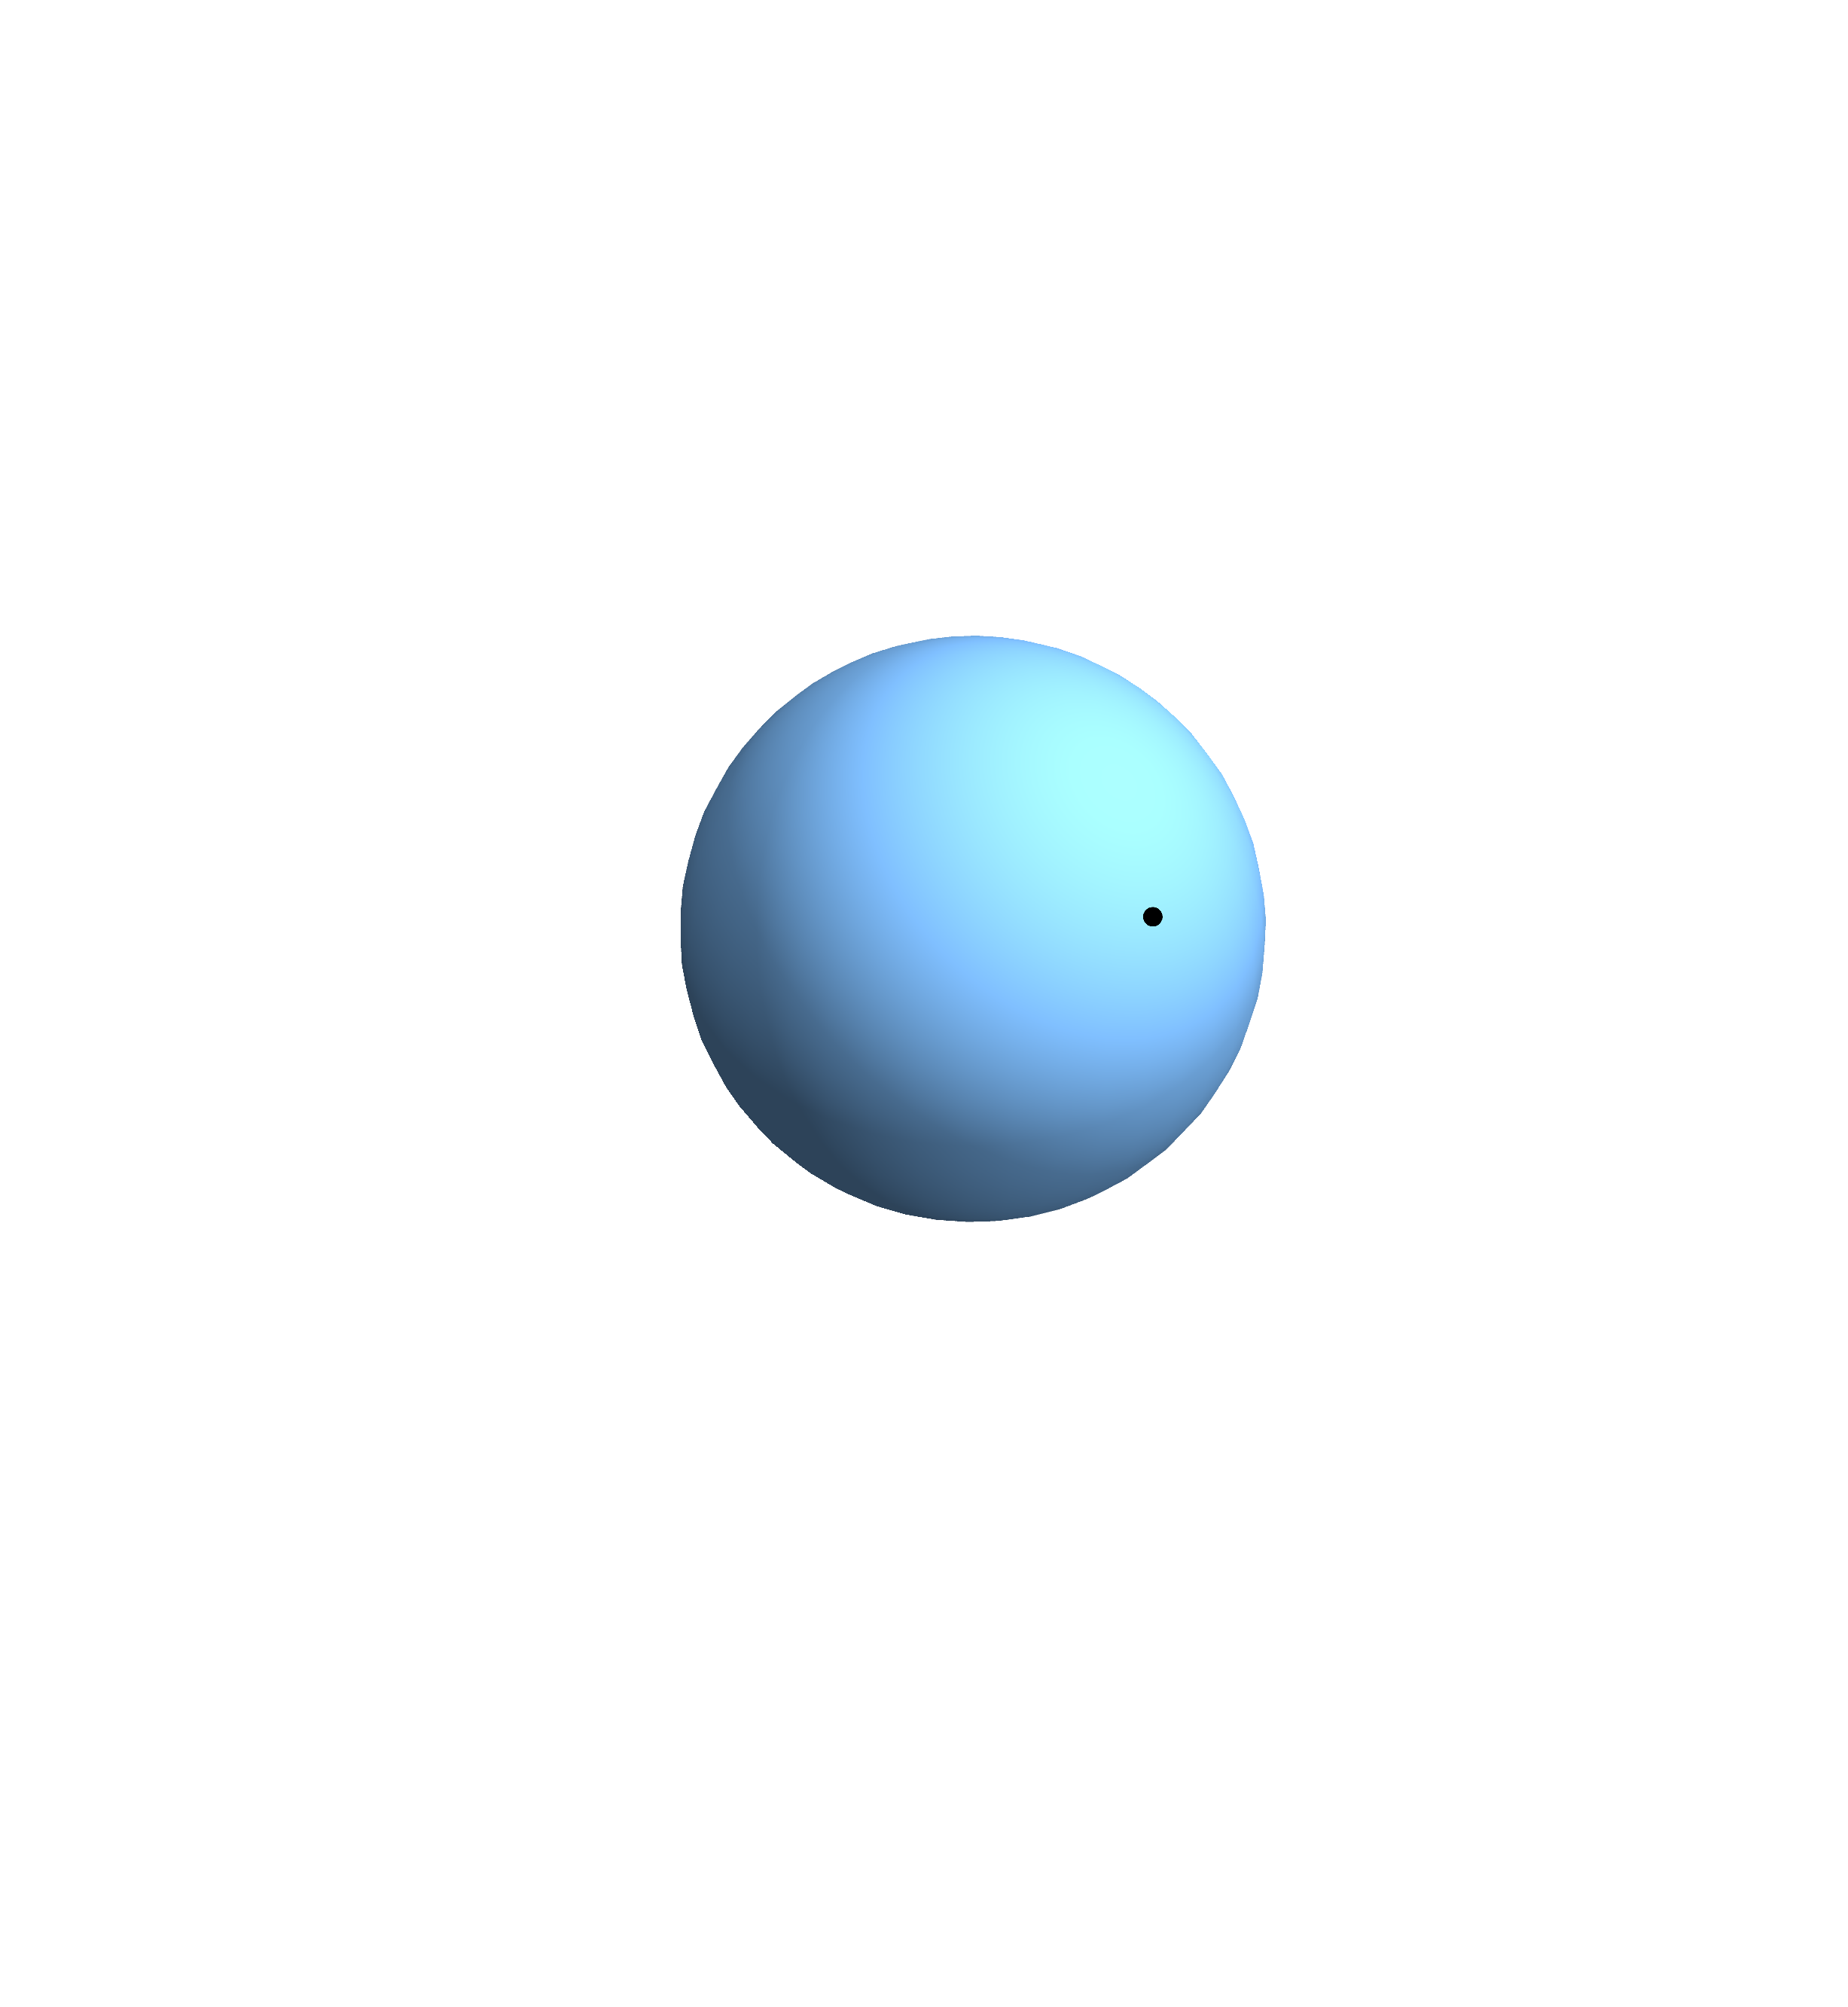
\includegraphics[clip, trim={13cm 15cm 8.5cm 11cm}, width=\textwidth * 35 / 100]{5 one satellite moved.pdf}}%
    \only<6>{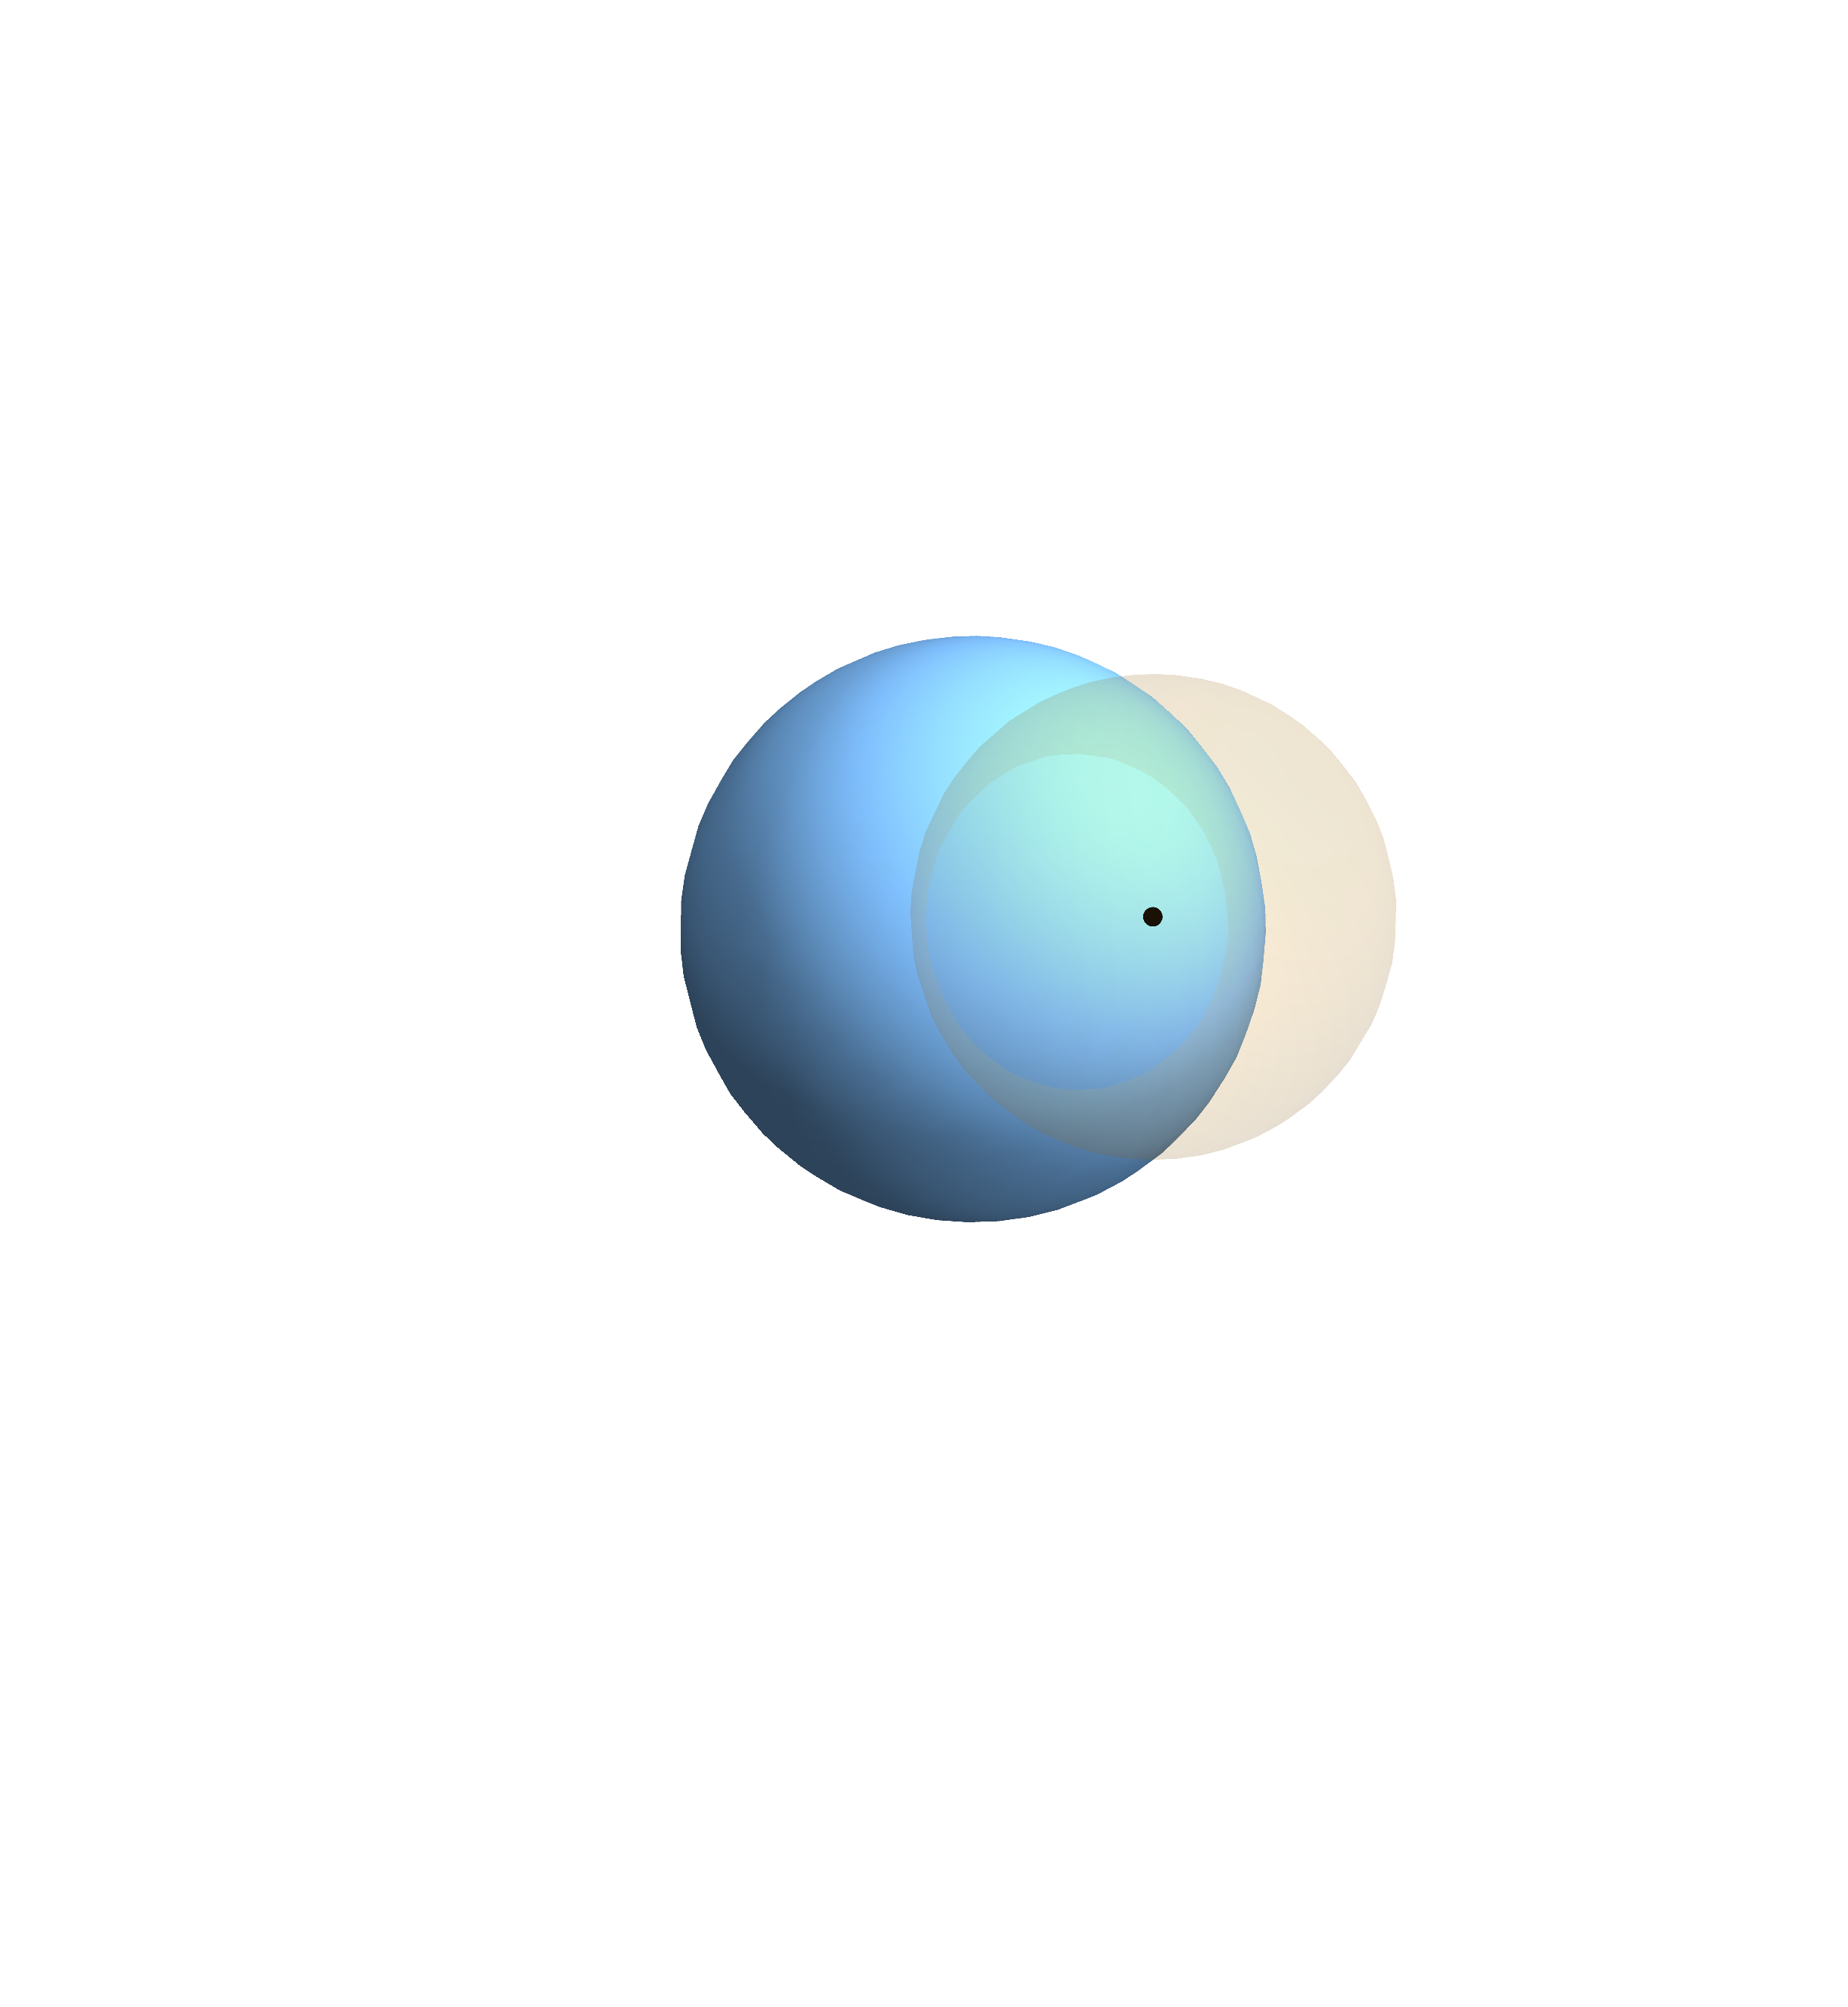
\includegraphics[clip, trim={13cm 15cm 8.5cm 11cm}, width=\textwidth * 35 / 100]{6 one satellite signal sphere.pdf}}%
    \only<7->{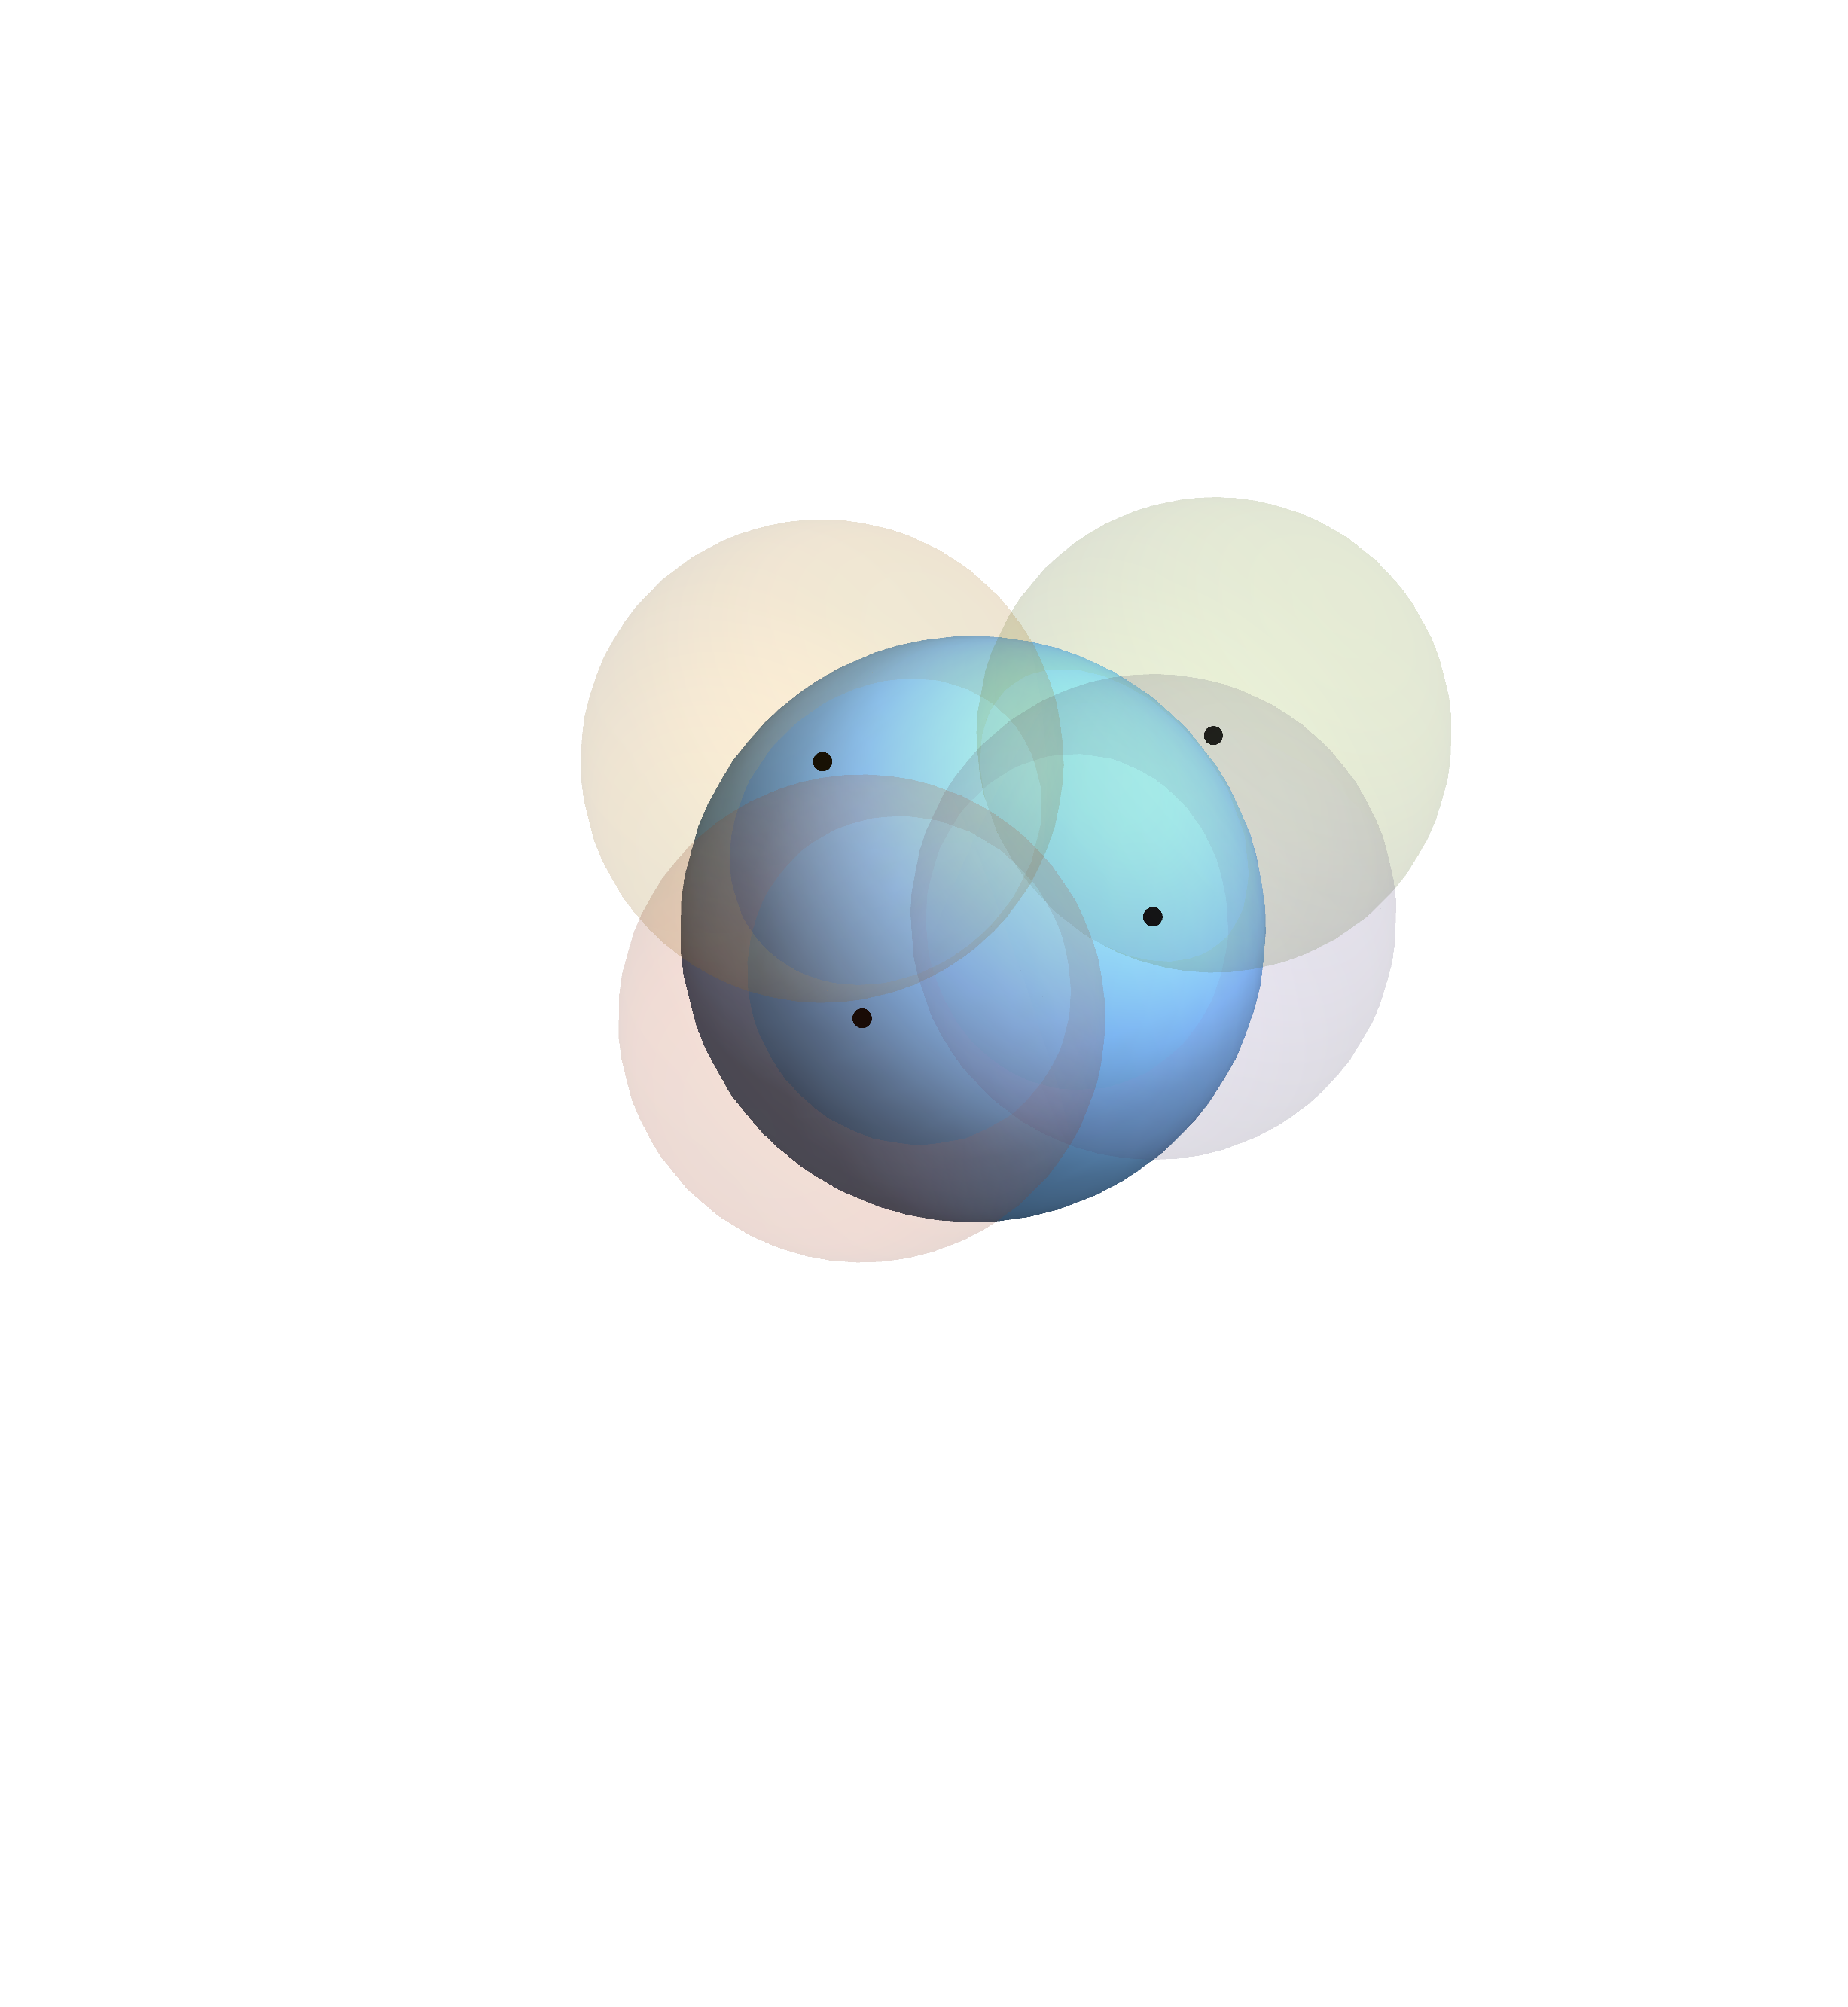
\includegraphics[clip, trim={13cm 15cm 8.5cm 11cm}, width=\textwidth * 35 / 100]{7 four satellites signal sphere.pdf}}%
    \onslide<4->{
        \begin{align*}
            T &= t_\text{received} - t_\text{transmitted}
            \onslide<5->{\\ d &= c T}
        \end{align*}
    }
    \onslide<8>{
        \begin{tikzpicture}[remember picture, overlay]
            \node[shift={(0cm, 1.85cm)}] at (current page.center) {
                
\includegraphics[width=1cm]{8 pin.png}
            };
        \end{tikzpicture}
    }
\end{frame}

\begin{frame}
    \frametitle{Overview of series}

    \begin{itemize}
        \item<2-> Theory
        
        \begin{enumerate}
            \setcounter{enumi}{1}

            \item<3-> Correlation
           
            \item<4-> GPS signals
        \end{enumerate}

        \item<5-> Stages
        
        \begin{enumerate}
            \setcounter{enumi}{3}

            \item<6-> Sampling
            
            \item<7-> Acquisition
            
            \item<8-> Tracking
            
            \item<9-> Decoding
            
            \item<10-> Solving
        \end{enumerate}
    \end{itemize}
\end{frame}

\end{document}